\documentclass{../../../../style/mkimain}

\series{4}
\month{květen}
\year{2023}

\begin{document}
%<*header>
\section*{IV.U3 Molekuly, molekuly, hejbejte se!}
%</header>
%<*task>

\noindent
\begin{enumerate}
    \item Které molekule pravděpodobně patří níže zobrazené Ramanovo spektrum? 
      \begin{choices}
        \choice \ce{H_2O}
        \choice \ce{CO_2}
        \choice \ce{CH_4}
        \choice \ce{O_3}
      \end{choices}
      \begin{center}
        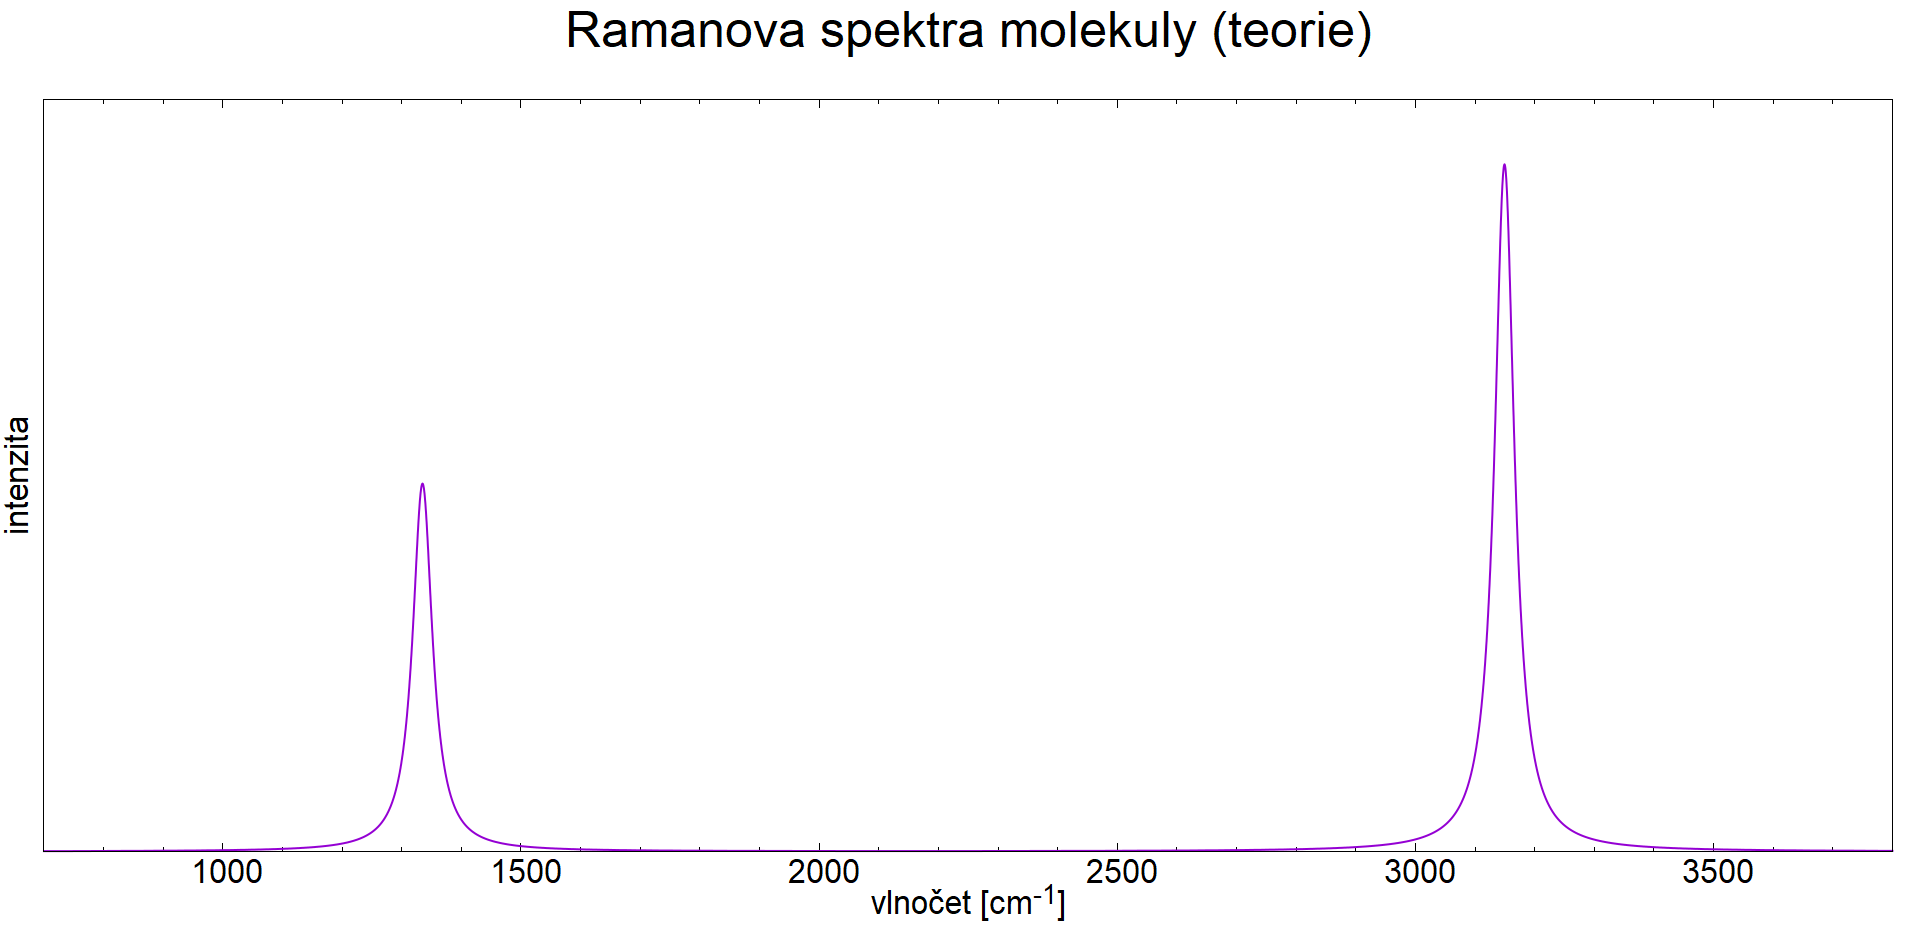
\includegraphics[width=\linewidth]{raman.png}
      \end{center}
    \item Co v molekule určuje toto (čistě Ramanovo) spektrum?
      \begin{choices}
        \choice Energetické hladiny přeskakujících elektronů
        \choice Energetické hladiny kmitajících jader
      \end{choices}
    \end{enumerate}
%</task> 
\end{document}
